\section{MoR：让不同 token 使用不同递归深度}
\label{sec:mixture-of-recursions}

本章的核心判断是：固定递归步数把所有 token 当成同样困难的问题处理，计算上很粗糙。混合递归（Mixture-of-Recursions, MoR）的目标，是让简单 token 提前结束，让复杂 token 获得更多内部更新；它把“递归深度”从全局超参数变成 token 级别的路由决策。

\begin{importantbox}{本章主张}
MoR 的关键收益来自计算分配，而非凭空减少推理难度。路由器（router）负责判断每个 token 需要多少递归；判断越早，执行越规整；判断越晚，适应性越强，训练和稳定性也更麻烦。
\end{importantbox}

\subsection{固定递归的低效性}

视频在 00:11:01--00:11:22 指出一个直接问题：即使循环模型能提供内部推理，所有 token 仍会经过相同数量的递归。简单词、标点、已经确定的上下文位置，和真正需要多步整合的 token 被分配同样计算量；这会把递归深度的优势变成新的浪费。

从第一性原理看，固定递归的成本可以写得很简单。若序列中有 \(n\) 个 token，每个 token 都运行最大递归步数 \(R\)，总计算量大致随 \(nR\) 增长。

\[
C_{\mathrm{fixed}}\propto nR
\]

符号说明：
\begin{itemize}
  \item \(C_{\mathrm{fixed}}\)：固定递归方案的近似计算量。
  \item \(n\)：序列中的 token 数。
  \item \(R\)：每个 token 都被迫执行的递归步数。
  \item \(\propto\)：正比关系，表示这里只讨论主导趋势。
\end{itemize}

这条公式的含义很朴素：当 \(R=3\) 时，每个 token 都要付三轮计算成本。若其中一半 token 只需要一轮就够，固定方案仍然会让它们跑满三轮。

\subsection{Token-choice：循环前的预分配路由}

MoR 引入路由器，让模型决定每个 token 实际需要的递归次数。视频在 00:11:42--00:12:00 展示的第一种方式是 token-choice routing（预分配路由）：循环开始前，路由器把每个 token 分到某个递归深度桶。图中每个 token 从底部进入 router，再被分配到 \(d=1\)、\(d=2\)、\(d=3\) 等深度。

先用白话解释公式：对第 \(i\) 个 token，路由器读取它初始隐藏状态 \(h_{i,0}\)，一次性预测需要运行的递归深度 \(d_i\)。预测完成后，计算路径就固定了。

\[
d_i=g_\phi(h_{i,0}),\qquad d_i\in\{1,\ldots,R\}
\]

符号说明：
\begin{itemize}
  \item \(i\)：token 的位置编号。
  \item \(h_{i,0}\)：第 \(i\) 个 token 在进入递归前的初始隐藏状态。
  \item \(g_\phi\)：路由器函数，\(\phi\) 是路由器参数。
  \item \(d_i\)：第 \(i\) 个 token 被分配的递归深度。
  \item \(R\)：允许的最大递归步数。
\end{itemize}

\begin{figure}[htbp]
  \centering
  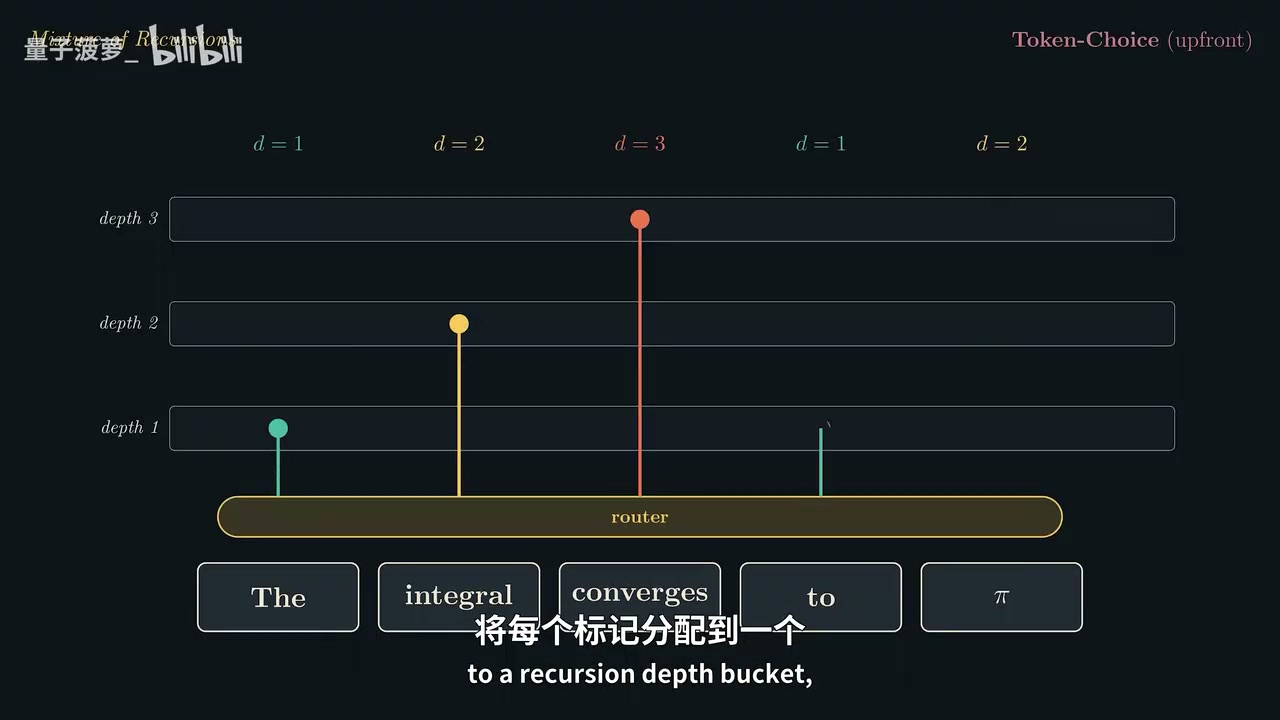
\includegraphics[width=0.82\linewidth,height=0.36\textheight,keepaspectratio]{figures/fig_11_token_choice_routing.jpg}
  \caption{Token-choice 预分配路由：每个 token 在循环开始前被分到递归深度桶，执行路径规整，代价是依赖早期难度判断。\protect\footnotemark}
  \label{fig:mor-token-choice-routing}
\end{figure}
\footnotetext{视频画面时间区间：00:11:42--00:12:00。}

这种方式的工程优点很清楚：路径从一开始就固定，调度更容易，批处理更整齐。主要风险也同样清楚：如果初始状态还没有足够信息判断 token 难度，早期误判后面很难纠正。视频在 00:11:53--00:12:00 正是这样描述它的限制。

\subsection{Expert-choice：递归过程中的逐步退出}

第二种方式是 expert-choice routing（逐步路由）。视频在 00:12:00--00:12:20 说明，模型在每次迭代时可以选择继续或退出。图中 token 会在不同深度处出现 exit 决策，路径随递归过程逐步确定。

先用白话解释公式：第 \(i\) 个 token 在第 \(t\) 次递归后，路由器根据当前状态 \(h_{i,t}\) 判断继续还是退出。因为 \(h_{i,t}\) 已经包含前几轮更新后的信息，这种判断通常比只看初始状态更灵活。

\[
a_{i,t}=g_\phi(h_{i,t}),\qquad a_{i,t}\in\{\mathrm{continue},\mathrm{exit}\}
\]

符号说明：
\begin{itemize}
  \item \(a_{i,t}\)：第 \(i\) 个 token 在第 \(t\) 步的路由动作。
  \item \(h_{i,t}\)：第 \(i\) 个 token 在第 \(t\) 次递归后的隐藏状态。
  \item \(g_\phi\)：逐步路由器函数。
  \item \(\mathrm{continue}\)：继续进入下一轮递归。
  \item \(\mathrm{exit}\)：退出递归，停止为该 token 分配后续循环计算。
\end{itemize}

\begin{figure}[htbp]
  \centering
  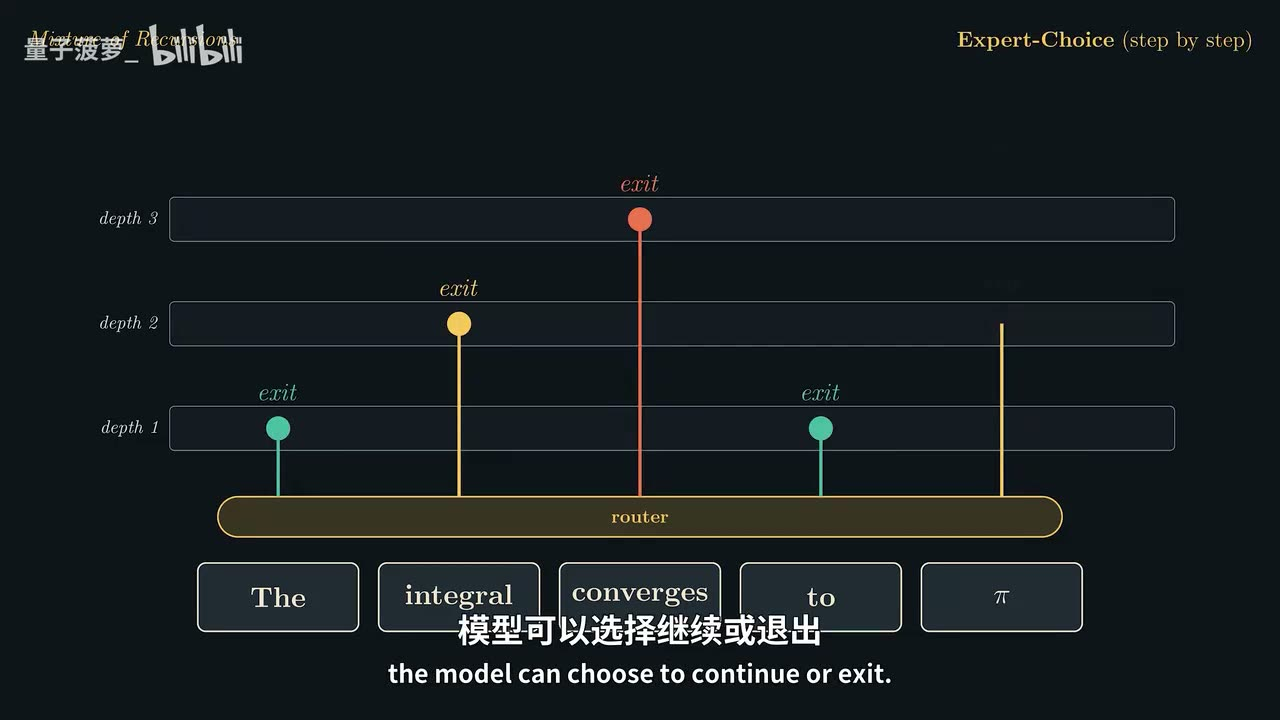
\includegraphics[width=0.82\linewidth,height=0.36\textheight,keepaspectratio]{figures/fig_12_expert_choice_routing.jpg}
  \caption{Expert-choice 逐步路由：token 可在每轮递归后选择继续或退出，适应性更强，训练与调度也更复杂。\protect\footnotemark}
  \label{fig:mor-expert-choice-routing}
\end{figure}
\footnotetext{视频画面时间区间：00:12:05--00:12:20。}

逐步路由的优势来自“边计算边判断”。当模型完成一两轮更新后，某些 token 的表示已经足够稳定，继续递归收益很低；另一些 token 仍处在关系整合阶段，需要更多更新。这个机制更贴近按需计算，但每一步都要做路由决策，也会让训练目标、负载均衡、梯度稳定和批处理效率变得更难处理。

\subsection{自适应计算量：MoR 的节省从哪里来}

MoR 的成本直觉可以用一条公式压缩：每个 token 只支付自己实际使用的递归深度。若第 \(i\) 个 token 的深度是 \(d_i\)，总计算量随所有 \(d_i\) 之和增长。

\[
C_{\mathrm{MoR}}\propto \sum_{i=1}^{n}d_i,\qquad C_{\mathrm{MoR}}\le C_{\mathrm{fixed}}\ \mathrm{when}\ d_i\le R
\]

符号说明：
\begin{itemize}
  \item \(C_{\mathrm{MoR}}\)：MoR 的近似计算量。
  \item \(n\)：序列中的 token 数。
  \item \(d_i\)：第 \(i\) 个 token 实际使用的递归深度。
  \item \(R\)：固定递归方案中的最大递归步数。
  \item \(C_{\mathrm{fixed}}\)：所有 token 都运行 \(R\) 步时的近似计算量。
\end{itemize}

这条公式的教学意义是：MoR 的收益不来自“循环本身免费”，而来自把递归步数集中给更需要的 token。若所有 token 最后都跑满 \(R\)，MoR 没有节省；若大量 token 早退，节省才会出现。

\begin{knowledgebox}{路由器直觉}
可以把 MoR 想成考场里的分题时间管理。简单题一眼能做完，就不该占用整张卷子的时间；难题需要多轮推导，可以拿更多时间。固定递归像每道题强制写满三页草稿，MoR 则把草稿纸按题目难度分配。
\end{knowledgebox}

\subsection{视频给出的路由对比与必要谨慎}

视频在 00:12:20--00:12:48 给出的对比是：在相同的三递归设置下，逐步版本被称为 expert-choice routing，平均少样本准确率约为 \(42.6\%\)；前期分配版本被称为 token-choice routing，约为 \(40\%\)。讲义应把这写成视频给出的对比，而非普遍定律。原因有三点。

第一，字幕和口播可能简化了论文术语，routing 名称与具体实现需要最终由画面或原论文确认。第二，\(42.6\%\) 与 \(40\%\) 是特定设置下的视频叙述，不能推出 expert-choice 在所有任务、模型规模和递归深度下都更好。第三，token-choice 的理论整洁性和工程调度优势仍然存在，数值落后可能来自早期难度预测过难、训练配置、任务类型或评价设置。

\begin{warningbox}{指标解读边界}
本章沿用视频画面和口播中的 routing 名称：token-choice 表示循环前预分配，expert-choice 表示逐步继续或退出。数值部分应写作“视频给出的对比是 expert-choice 约 \(42.6\%\)，token-choice 约 \(40\%\)”；在最终整合前，若要写成论文级结论，需要核验原论文表格与指标定义。
\end{warningbox}

\subsection{本章小结}

本章把循环模型的效率问题从“是否能多想几轮”推进到“哪些 token 值得多想”。读者应带走三点：第一，固定递归会让简单 token 和复杂 token 支付同样计算成本；第二，token-choice 在循环前预分配深度，执行规整但依赖早期判断；第三，expert-choice 在递归过程中逐步决定继续或退出，更灵活也更难训练。视频给出的 \(42.6\%\) 与 \(40\%\) 对比只能作为该视频语境下的指标线索，不能被扩展成无条件的路由优劣结论。下一章需要继续处理真实推理系统里的 KV cache，因为节省参数和递归步数之后，内存带宽仍会追上来。
